
\begin{figure*}
\centering
\subfloat[\Process~$R$ efficiently advertises its content using epidemic propagation. Every \process requests $R$ if needed.\label{fig:partition_intuitionA}]{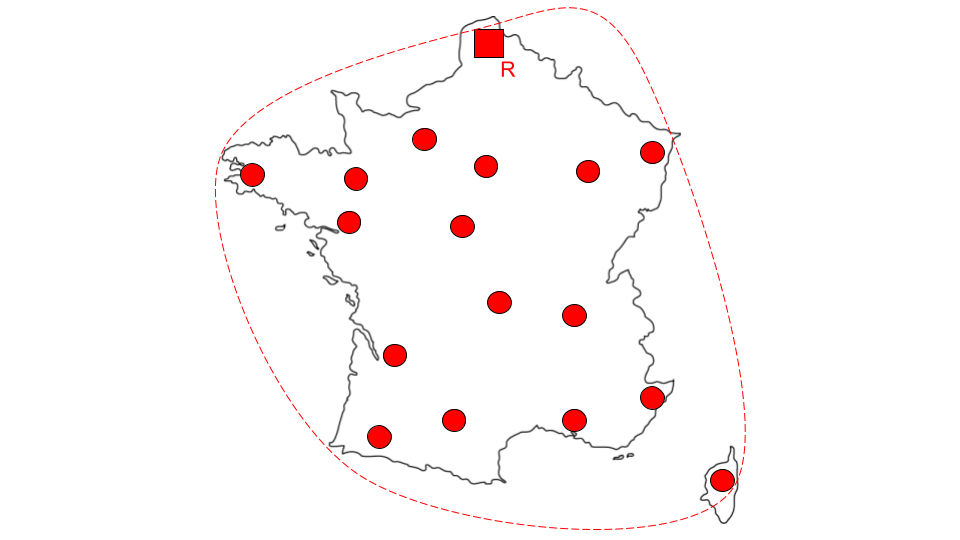
\includegraphics[trim=6cm 0.33cm 6cm 0.33cm, clip, width=0.24\textwidth]{img/Dynamic-partitioning-1.png}}
\hfill
\subfloat[\Process $G$ creates a second replica splitting the red set in two. \Processes request their closest replica host.\label{fig:partition_intuitionB}]{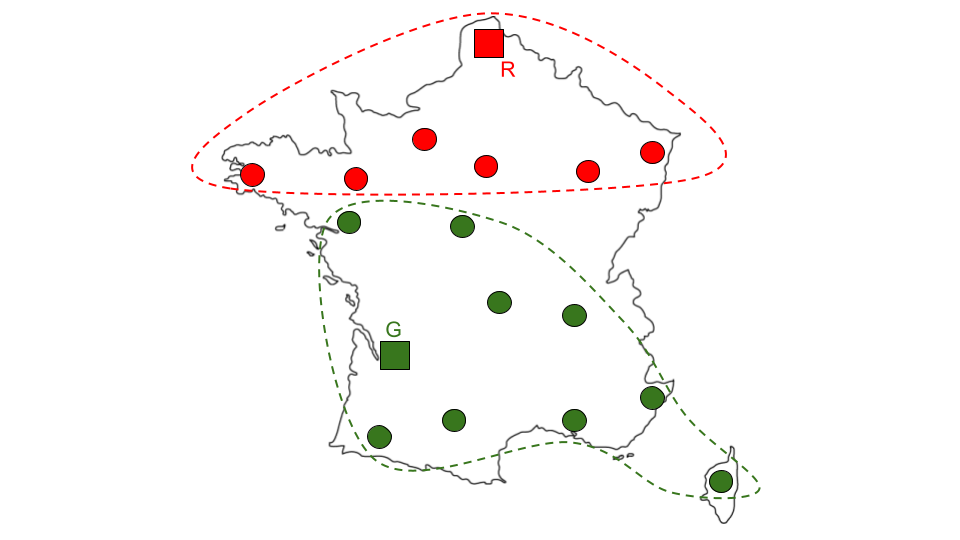
\includegraphics[trim=6cm 0.33cm 6cm 0.33cm, clip, width=0.24\textwidth]{img/Dynamic-partitioning-2.png}}\hfill
\subfloat[\Process $B$ creates another replica. \Process~$B$ needs to notify only a small subset of \processes.\label{fig:partition_intuitionC}]{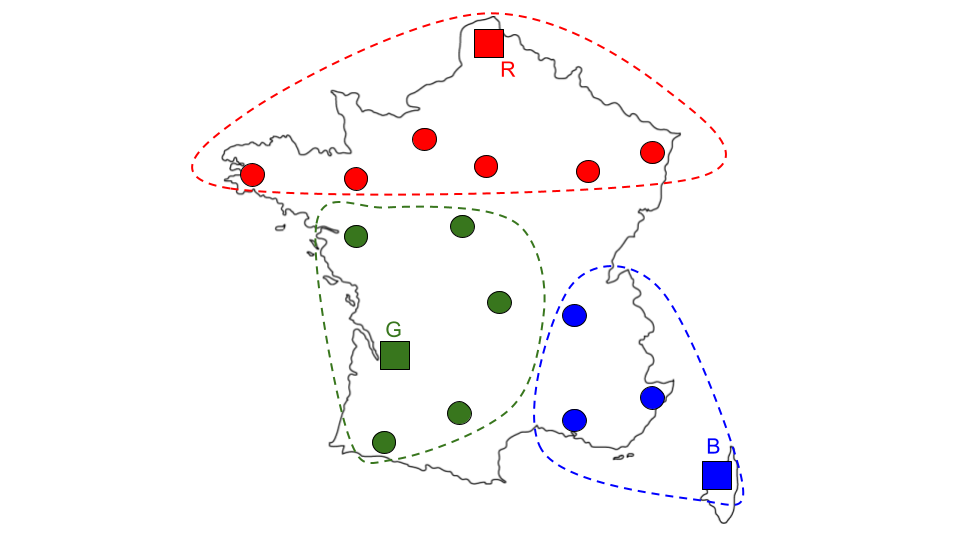
\includegraphics[trim=6cm 0.33cm 6cm 0.33cm, clip, width=0.24\textwidth]{img/Dynamic-partitioning-3.png}}\hfill
\subfloat[\Process $G$ destroys its replica. \Processes that belonged to its partition must find the closest partition they are in.\label{fig:partition_intuitionD}]{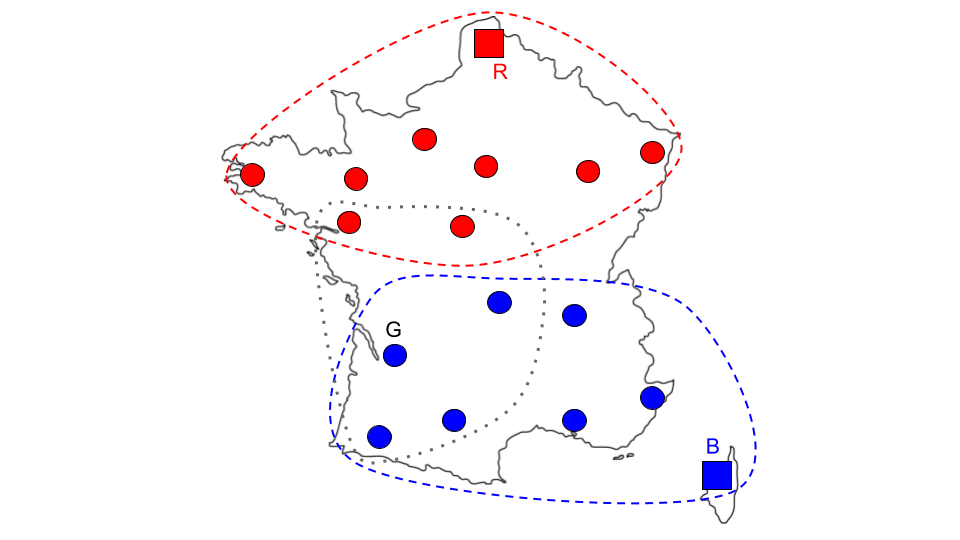
\includegraphics[trim=6cm 0.33cm 6cm 0.33cm, clip, width=0.24\textwidth]{img/Dynamic-partitioning-4.png}}
%
\caption{The french RENATER topology. Partitions
  grow and shrink depending on creations and removals of
  replicas.} \label{fig:partition_intuition}
\end{figure*}

%%% Local Variables: 
%%% mode: latex
%%% TeX-master: "../paper"
%%% ispell-local-dictionary: "english"
%%% End: 
